\documentclass{standalone}
\usepackage{tikz}
\usetikzlibrary{patterns, positioning}

\begin{document}
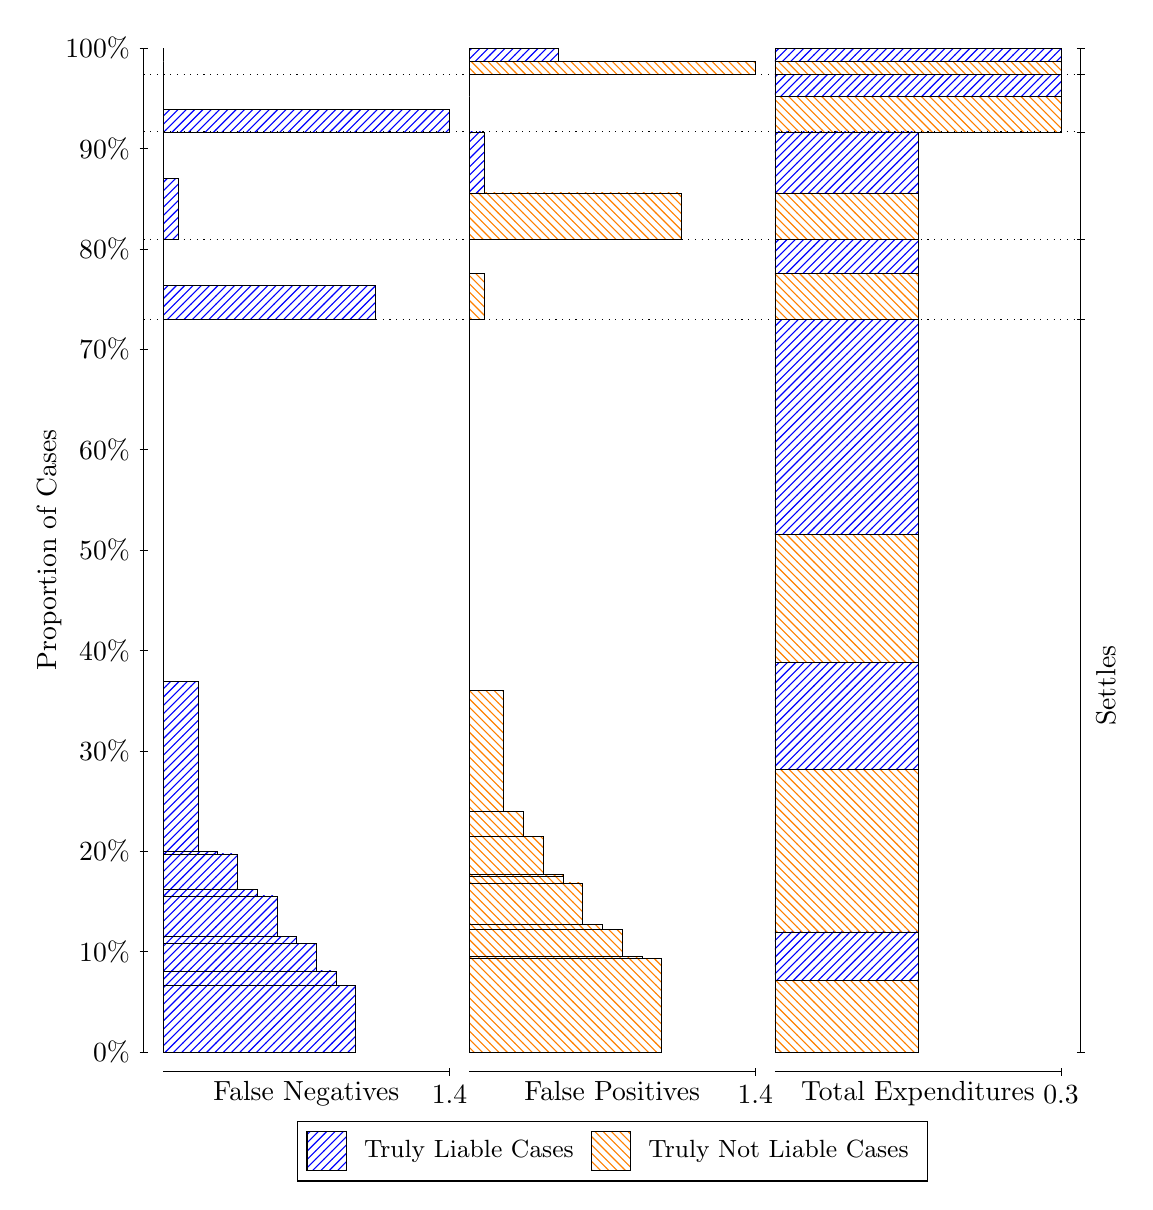
\begin{tikzpicture}
\draw[black, very thin] (1.5,1.75) -- (1.5,14.5);
\node[rotate=90, anchor=center] at (0.3, 8.125) {Proportion of Cases};
\draw[black, very thin] (1.45,1.75) -- (1.55,1.75);
\node[anchor=east] at (1.45, 1.75) {0\%};
\draw[black, very thin] (1.45,3.025) -- (1.55,3.025);
\node[anchor=east] at (1.45, 3.025) {10\%};
\draw[black, very thin] (1.45,4.3) -- (1.55,4.3);
\node[anchor=east] at (1.45, 4.3) {20\%};
\draw[black, very thin] (1.45,5.575) -- (1.55,5.575);
\node[anchor=east] at (1.45, 5.575) {30\%};
\draw[black, very thin] (1.45,6.85) -- (1.55,6.85);
\node[anchor=east] at (1.45, 6.85) {40\%};
\draw[black, very thin] (1.45,8.125) -- (1.55,8.125);
\node[anchor=east] at (1.45, 8.125) {50\%};
\draw[black, very thin] (1.45,9.4) -- (1.55,9.4);
\node[anchor=east] at (1.45, 9.4) {60\%};
\draw[black, very thin] (1.45,10.675) -- (1.55,10.675);
\node[anchor=east] at (1.45, 10.675) {70\%};
\draw[black, very thin] (1.45,11.95) -- (1.55,11.95);
\node[anchor=east] at (1.45, 11.95) {80\%};
\draw[black, very thin] (1.45,13.225) -- (1.55,13.225);
\node[anchor=east] at (1.45, 13.225) {90\%};
\draw[black, very thin] (1.45,14.5) -- (1.55,14.5);
\node[anchor=east] at (1.45, 14.5) {100\%};

\draw[black, very thin] (13.4,1.75) -- (13.4,14.5);
\draw[black, very thin] (13.35,1.75) -- (13.45,1.75);
\node[anchor=west] at (13.35, 1.75) {};
\draw[black, very thin] (13.35,11.053) -- (13.45,11.053);
\node[anchor=west] at (13.35, 11.053) {};
\draw[black, very thin] (13.35,12.067) -- (13.45,12.067);
\node[anchor=west] at (13.35, 12.067) {};
\draw[black, very thin] (13.35,13.436) -- (13.45,13.436);
\node[anchor=west] at (13.35, 13.436) {};
\draw[black, very thin] (13.35,14.167) -- (13.45,14.167);
\node[anchor=west] at (13.35, 14.167) {};
\draw[black, very thin] (13.35,14.5) -- (13.45,14.5);
\node[anchor=west] at (13.35, 14.5) {};

\draw[black, very thin, pattern color=blue, pattern=north east lines] (1.75,1.75) rectangle (4.1931,2.5937);
\draw[black, very thin, pattern color=blue, pattern=north east lines] (1.75,2.5937) rectangle (3.9425,2.7788);
\draw[black, very thin, pattern color=blue, pattern=north east lines] (1.75,2.7788) rectangle (3.692,3.1313);
\draw[black, very thin, pattern color=blue, pattern=north east lines] (1.75,3.1313) rectangle (3.4414,3.2143);
\draw[black, very thin, pattern color=blue, pattern=north east lines] (1.75,3.2143) rectangle (3.1908,3.7337);
\draw[black, very thin, pattern color=blue, pattern=north east lines] (1.75,3.7337) rectangle (2.9402,3.8101);
\draw[black, very thin, pattern color=blue, pattern=north east lines] (1.75,3.8101) rectangle (2.6897,4.2663);
\draw[black, very thin, pattern color=blue, pattern=north east lines] (1.75,4.2663) rectangle (2.4391,4.2989);
\draw[black, very thin, pattern color=blue, pattern=north east lines] (1.75,4.2989) rectangle (2.1885,6.4607);
\draw[black, very thin, pattern color=orange, pattern=north west lines] (1.75,6.4607) rectangle (1.75,11.053);
\draw[black, very thin, pattern color=blue, pattern=north east lines] (1.75,11.053) rectangle (4.4437,11.483);
\draw[black, very thin, pattern color=orange, pattern=north west lines] (1.75,11.483) rectangle (1.75,12.067);
\draw[black, very thin, pattern color=blue, pattern=north east lines] (1.75,12.067) rectangle (1.9379,12.844);
\draw[black, very thin, pattern color=orange, pattern=north west lines] (1.75,12.844) rectangle (1.75,13.436);
\draw[black, very thin, pattern color=blue, pattern=north east lines] (1.75,13.436) rectangle (5.3833,13.721);
\draw[black, very thin, pattern color=orange, pattern=north west lines] (1.75,13.721) rectangle (1.75,14.167);
\draw[black, very thin, pattern color=orange, pattern=north west lines] (1.75,14.167) rectangle (1.75,14.327);
\draw[black, very thin, pattern color=blue, pattern=north east lines] (1.75,14.327) rectangle (1.75,14.5);
\draw[black, very thin, pattern color=orange, pattern=north west lines] (5.6333,1.75) rectangle (8.0764,2.9424);
\draw[black, very thin, pattern color=orange, pattern=north west lines] (5.6333,2.9424) rectangle (7.8259,2.9681);
\draw[black, very thin, pattern color=orange, pattern=north west lines] (5.6333,2.9681) rectangle (7.5753,3.3057);
\draw[black, very thin, pattern color=orange, pattern=north west lines] (5.6333,3.3057) rectangle (7.3247,3.3746);
\draw[black, very thin, pattern color=orange, pattern=north west lines] (5.6333,3.3746) rectangle (7.0741,3.8965);
\draw[black, very thin, pattern color=orange, pattern=north west lines] (5.6333,3.8965) rectangle (6.8236,3.9873);
\draw[black, very thin, pattern color=orange, pattern=north west lines] (5.6333,3.9873) rectangle (6.8236,4.0039);
\draw[black, very thin, pattern color=orange, pattern=north west lines] (5.6333,4.0039) rectangle (6.573,4.4909);
\draw[black, very thin, pattern color=orange, pattern=north west lines] (5.6333,4.4909) rectangle (6.3224,4.8018);
\draw[black, very thin, pattern color=orange, pattern=north west lines] (5.6333,4.8018) rectangle (6.0718,6.3425);
\draw[black, very thin, pattern color=blue, pattern=north east lines] (5.6333,6.3425) rectangle (5.6333,11.053);
\draw[black, very thin, pattern color=orange, pattern=north west lines] (5.6333,11.053) rectangle (5.8213,11.637);
\draw[black, very thin, pattern color=blue, pattern=north east lines] (5.6333,11.637) rectangle (5.6333,12.067);
\draw[black, very thin, pattern color=orange, pattern=north west lines] (5.6333,12.067) rectangle (8.327,12.659);
\draw[black, very thin, pattern color=blue, pattern=north east lines] (5.6333,12.659) rectangle (5.8213,13.436);
\draw[black, very thin, pattern color=orange, pattern=north west lines] (5.6333,13.436) rectangle (5.6333,13.882);
\draw[black, very thin, pattern color=blue, pattern=north east lines] (5.6333,13.882) rectangle (5.6333,14.167);
\draw[black, very thin, pattern color=orange, pattern=north west lines] (5.6333,14.167) rectangle (9.2667,14.327);
\draw[black, very thin, pattern color=blue, pattern=north east lines] (5.6333,14.327) rectangle (6.7609,14.5);
\draw[black, very thin, pattern color=orange, pattern=north west lines] (9.5167,1.75) rectangle (11.333,2.6553);
\draw[black, very thin, pattern color=blue, pattern=north east lines] (9.5167,2.6553) rectangle (11.333,3.2759);
\draw[black, very thin, pattern color=orange, pattern=north west lines] (9.5167,3.2759) rectangle (11.333,5.3386);
\draw[black, very thin, pattern color=blue, pattern=north east lines] (9.5167,5.3386) rectangle (11.333,6.7016);
\draw[black, very thin, pattern color=orange, pattern=north west lines] (9.5167,6.7016) rectangle (11.333,8.3262);
\draw[black, very thin, pattern color=blue, pattern=north east lines] (9.5167,8.3262) rectangle (11.333,11.053);
\draw[black, very thin, pattern color=orange, pattern=north west lines] (9.5167,11.053) rectangle (11.333,11.637);
\draw[black, very thin, pattern color=blue, pattern=north east lines] (9.5167,11.637) rectangle (11.333,12.067);
\draw[black, very thin, pattern color=orange, pattern=north west lines] (9.5167,12.067) rectangle (11.333,12.659);
\draw[black, very thin, pattern color=blue, pattern=north east lines] (9.5167,12.659) rectangle (11.333,13.436);
\draw[black, very thin, pattern color=orange, pattern=north west lines] (9.5167,13.436) rectangle (13.15,13.882);
\draw[black, very thin, pattern color=blue, pattern=north east lines] (9.5167,13.882) rectangle (13.15,14.167);
\draw[black, very thin, pattern color=orange, pattern=north west lines] (9.5167,14.167) rectangle (13.15,14.327);
\draw[black, very thin, pattern color=blue, pattern=north east lines] (9.5167,14.327) rectangle (13.15,14.5);
\draw[black, dotted] (1.5,11.053) -- (13.4,11.053);
\draw[black, dotted] (1.5,12.067) -- (13.4,12.067);
\draw[black, dotted] (1.5,13.436) -- (13.4,13.436);
\draw[black, dotted] (1.5,14.167) -- (13.4,14.167);
\draw[black, very thin] (1.75,1.5) -- (5.3833,1.5);
\node[anchor=north] at (3.5667, 1.5) {False Negatives};
\draw[black, very thin] (5.3833,1.45) -- (5.3833,1.55);
\node[anchor=north] at (5.3833, 1.45) {1.4};

\draw[black, very thin] (5.6333,1.5) -- (9.2667,1.5);
\node[anchor=north] at (7.45, 1.5) {False Positives};
\draw[black, very thin] (9.2667,1.45) -- (9.2667,1.55);
\node[anchor=north] at (9.2667, 1.45) {1.4};

\draw[black, very thin] (9.5167,1.5) -- (13.15,1.5);
\node[anchor=north] at (11.333, 1.5) {Total Expenditures};
\draw[black, very thin] (13.15,1.45) -- (13.15,1.55);
\node[anchor=north] at (13.15, 1.45) {0.3};

\node[black, centered, rotate=90] at (13.72, 6.4016) {Settles};





\draw (7.449999999999999,1.5) node[draw=none] (baseCoordinate) {};
\begin{scope}[align=center]
        \matrix[scale=0.5, draw=black, below=0.5cm of baseCoordinate, nodes={draw}, column sep=0.1cm]{
            \node[rectangle, draw, minimum width=0.5cm, minimum height=0.5cm, pattern=north east lines, pattern color=blue] {}; &
            \node[draw=none, font=\small] (B) {Truly Liable Cases}; &
            \node[rectangle, draw, minimum width=0.5cm, minimum height=0.5cm, pattern=north west lines, pattern color=orange] {}; &
            \node[draw=none, font=\small] (B) {Truly Not Liable Cases}; \\
            };
\end{scope}

\end{tikzpicture}
\end{document}